\subsection{SEOSS evaluation with T5 PICARD}

After studying the SEOSS dataset, we decided to experiment with the PICARD model\ref{picard} to evaluate its performance against that of SQLNet and RatSQL. We decided to use the T5Base model for our experiment, as it is smaller than the T5-3B and T5-11B models used by most state-of-the-art studies. To ensure a fair comparison between the models, we used two beam sizes of 2 and 4 and the same evaluation metrics as SEOSS-SQLNet and SEOSS-RatSQL, which is "exact matching accuracy". We wanted to see if the PICARD model could achieve similar results to those of SQLNet and RatSQL, so we conducted our experiment with our findings. The results of our experiment are discussed in the following section and can be used to compare the performance of the PICARD model to the models used in the SEOSS study.
\footnote[1]{Link to the Github Page: \url{https://github.com/yazdipour/text-to-sql-seoss-t5}}

\begin{table}[!ht]
    \centering
    \begin{tabular}{|c|c|c|L|L|}
        \hline
        Model    & Picard Mode       & Beams & \textbf{Exact Matching Accuracy} & \textbf{Execution Accuracy} \\ \hline
        T5-base  & parse with guards & 2     & 0.3297                           & 0.3576                      \\ \hline
        T5-base  & lex               & 4     & 0.3071                           & 0.3039                      \\ \hline
        T5-base  & parse with guards & 4     & 0.3286                           & 0.3512                      \\ \hline
        T5-large & lex               & 2     & 0.3672                           & 0.3629                      \\ \hline
        T5-large & parse with guards & 4     & 0.4274                           & 0.4822                      \\ \hline
    \end{tabular}
    \caption{Expermiment Accuracy Results}
\end{table}

The table shows the results of various configurations of T5-base and T5-large models for natural language processing tasks. The configurations are differentiated by the Picard mode parse with guards or lex and the number of beams used in the beam search process 2 or 4.

Comparing the results, we can observe that:

The T5-large model generally performs better than the T5-base model in both exact matching accuracy and execution accuracy.
As we could have a predicate, the parse with guards Picard mode performs better than the lex Picard mode in both models. So we decided to continue only with parse with guards.
Using four beams instead of 2 in the beam search process improves the performance for both models and Picard modes.
The highest exact matching accuracy is achieved by the T5-large model with parse with guards Picard mode and four beams 0.4274.
The highest execution accuracy is also achieved by the T5-large model with parse with guards Picard mode and four beams 0.4822.
Increasing beam size does not have a significant effect compared to changing the model from base to large.
\subsubsection*{F1 Scores}

% add image here pics/ez/F1.svg
\begin{figure}[htb]
    \centering
    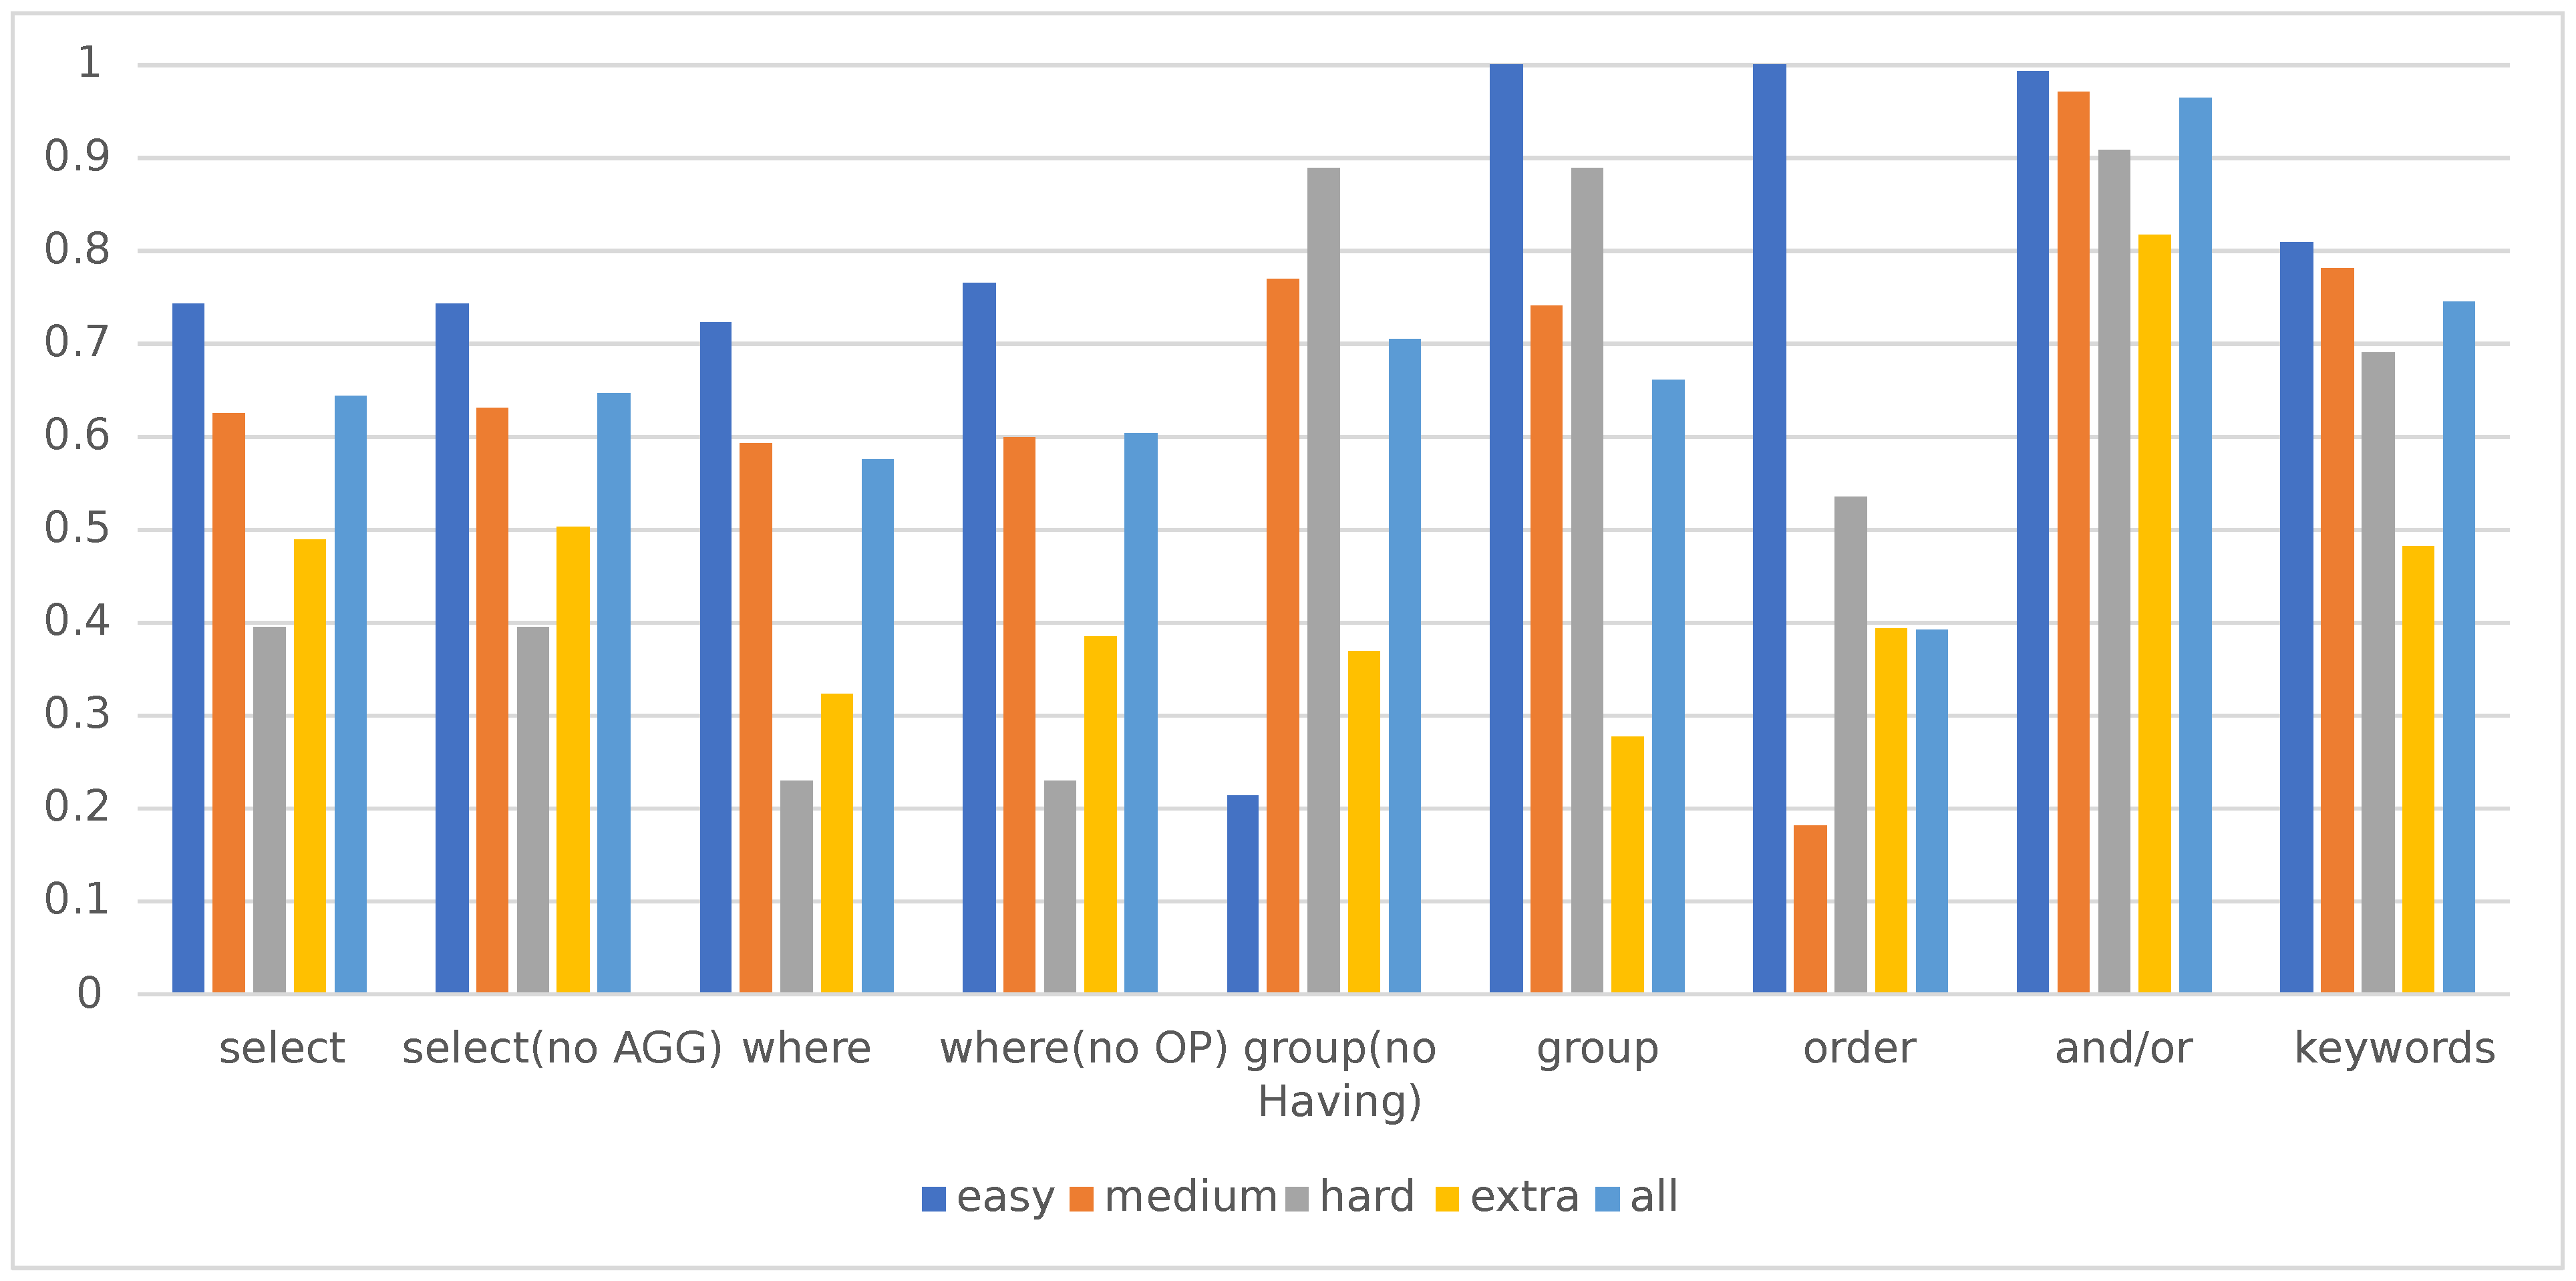
\includegraphics[width=1\textwidth]{pics/ez/F1eps}
    \caption{F1 Scores of Component Matching - PICARD T5-Large 4-Beam}
\end{figure}

Here, we can observe the F1 scores of each SQL Keyword for the PICARD T5-Large 4-Beam experiment on the SEOSS dataset. We can see that PICARD has managed to attain a very impressive F1 score for the SEOSS dataset without even having to be specifically trained for our dataset. This is a very encouraging result and indicates that the model is able to generalize accurately across different domains. Moreover, it is essential to note that the F1 score obtained by the PICARD model was obtained without any additional fine-tuning. This is a testament to the robustness and capability of the model and further highlights its ability to generalize to different datasets.

We experimented with a variety of different parameters, including beam size, modes and model sizes, and spent multiple hours for each evaluation. These experiments have been carefully documented in the Appendix of this thesis, where you can also find them in the project repository.
